\section{Comments on structure of proposal}

\begin{itemize}
\item Background: should be much broader, example applications
\begin{itemize}
\item Vesicles for drug delivery
\item Extracellular vesicles (EVs) are newly recognized as important vectors for carrying and spreading antibiotic resistance genes (ARGs)
\item Building with nanoparticles, from the bottom up
\item Motivation:
MD and continuum simulations are clumsy; work over limited time/length scales; we need a
a robust method to complement established methods and processes.
The present proposal is our first attempt at creating such a model.
\end{itemize}

\item Model formulation: put the applied math formulas up front; change name ``particle'' to something else
\item Numerics: discuss advantages and challenges if BIE

\item Summary of respective resumes/contributions to this area

\item Specific Aim 1: Measuring material properties of amphiphile self-assembly
\item Specific Aim 2: Efficient, high-order methods for large-scale simulations
\item Specific Aim 3: Coarse graining and continuum models

\item Broader Impacts
\item Intellectual Merit
\item Prior NSF support

\item Other notes: do not waste the CV and prior work section:
play up significance of works.
``In our JFM/Nature/Biophys J paper'', ``In our much noticed,'' ``In our highly cited/referenced'', ``Detailed modeling and simulation which is the crown jewel of
applied mathematics''.
Use suggested reviewers to our advantage. 

%Here is an interesting problem.
%Here is how it’s addressed.
%Here is what we are going to do. 

\end{itemize}


\noindent
{\bf Collaborative Research: Mathematical modeling and simulation of
self-assembling amphiphilic particles in solvent} \\
{\em Rolf Ryham (lead PI, Fordham University),
Bryan Quaife (PI, Florida State University), and
Yuan-Nan Young (PI, New Jersey Institute of Technology)}

\section{Background}
\label{sec:background}

\textbf{Very broad introduction}

\subsubsection{Problem formulation}
%\begin{wrapfigure}[h!]
\begin{wrapfigure}[11]{r}{0.55\textwidth}
 \centering
 \vspace{-3pt}
 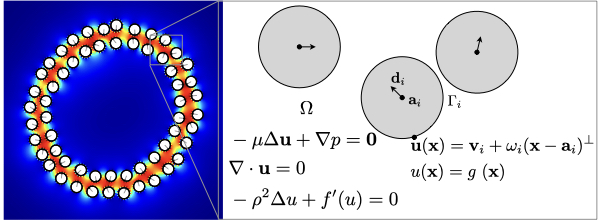
\includegraphics[width=0.55\textwidth]{figures/SpecificAim1/Domain.jpg}
 \caption{\label{fig:flow_map}
   In the HAP formulation,
   a system of exterior problems 
   defines the hydronamic and hydrophobic interactions.
   The colormap is for the intensity of $u$.
   The dynamics lead to self-organized structures like a vesicle bilayer.}
\end{wrapfigure}

The mathematical formulation is a nonlinear system for the dynamics of a
collection of particles. The interactions come from a system of 
partial differential equations (PDEs) that comprise hydrodynamic
interactions and hydrophobic interactions.
%The formulation prevents particle collisions through excluded volume
%potentials. 
The hydrodynamic interactions come from the mobility problem for rigid
particles immersed in a viscous solvent. We then use a
second-order Adams-Bashforth method to update the particle configuration.
Assuming inertial terms are
negligible, the particle motion is goverened by the Stokes equations
\begin{subequations}
  \label{eq:stokes}
  \begin{alignat}{3}
  \label{eq:stokes1}
  -\mu \Delta \uu + \nabla p &= \mathbf{0}, && \xx \in \Omega, \\
    \label{eq:stokes2}
  \nabla\cdot \uu &= 0, \qquad && \xx \in \Omega, \\
\label{eq:stokes3}
  \uu - \uu_\infty &\to \mathbf{0}, && |\xx| \to \infty,
  \end{alignat}
\end{subequations}
%\begin{alignat}{3}
%\label{eq:stokes1}
%  -\mu \Delta \uu + \nabla p &= \mathbf{0}, 
%    && \xx \in \Omega, \\
%\label{eq:stokes2}
%  \nabla\cdot \uu &= 0, \qquad && \xx \in \Omega, \\
%\label{eq:stokes3}
%  \uu - \uu_\infty &\to \mathbf{0}, && |\xx| \to \infty,
%\end{alignat}
%
where $\uu$ is the velocity and $p$ is the pressure of the solvent,
$\uu_\infty$ is the background flow, and $\mu$ is the constant solvent
viscosity. The domain $\Omega = \Omega(t)$ is the fluid region surrounding the
particles and changes shape as the particles move.
Since the particles are rigid, the solvent velocity satisfies
a no-slip boundary condition for a rigid body motion 
%\begin{align}
%\label{eq:rigid_bc}
%  \uu(\xx) = \vv_i + \omega_i  (\xx - \aa_i)^\perp, \quad
%    \xx \in \Gamma_i,\qquad  i=1,\ldots,N_p,
%\end{align}
on the particle boundary $\Gamma_i$ with translational velocity $\vv_i$
and angular velocity $\omega_i$ (Figure \ref{fig:flow_map}).
Given imposed forces acting on each
particle, the \emph{mobility problem} consists of finding
translational and angular velocities so that viscous fluid forces
balance the imposed forces.

The hydrophobic interactions come from the tendency of particles to
minimize the free energy of the structure of the surrounding water
molecules. The free energy functional takes the form 
\begin{equation}
\label{eq:free_energy}
  F[u] = C \int_{\Omega} \left(\rho |\nabla u|^2 + \rho^{-1} f(u)\right)
  \,d\xx,
\end{equation}
where $u$ is an order parameter for the structure of water, $\rho$ is a
decay length, $C$ is a constant, and $f(u)$ is a potential.
Hydrogen-bond persistence times are on the order of picoseconds
which is much smaller than characteristic time for 
particle motion \cite{MaGa13}.
Thus we assume $u$ minimizes $F[u]$ for all times.
Assuming appropriate conditions on $f(u)$ (\cite{evans10}, \S 8.2),
$u$ is bounded and satisfies the Euler-Lagrange equation
\begin{equation}
\label{eq:SL}
-\rho^2 \Delta u + \tfrac{1}{2}f'(u) = 0  \text{ in } \Omega,\quad u = g,
\text{ on } \bd\Omega.
\end{equation}
The boundary condition $g$ is a material label that is transported with
the particle (Figure~\ref{fig:bcs}).

The particles lower the free energy $F[u]$ of the surrounding water
by moving. We calculate the rate of change of $F[u]$ using
\emph{variation of the domain} ~\cite{Fu2018_SIAM,Bandle2015, Schiffer1954, Grinfeld2010}.
Carrying out
this variation yields a 
%The hydrophobic forces are torques are
%\begin{equation}
%  \label{eq:hydrophobicAttraction}
%  \FF_i^{\text{hydro}} = \int_{\Gamma_i} {\bf T}\cdot \nnu \, \dif s, 
%    \quad 
%    T_i^{\text{hydro}} = \int_{\Gamma_i} (\xx - \aa_i)^{\perp} \cdot
%    ({\bf T} \cdot \nnu) \dif s.
%\end{equation}
stress  
\begin{align}
  \label{eq:stress}
\mathbf{T}
= C \left[ \rho^{-1} f(u) \mathbf{I}
  + \rho \left(|\nabla u|^2 \mathbf{I} - 2\nabla u \nabla u^T\right)\right].
\end{align}
The imposed forces and torques come from the integration of $\mathbf{T}$
along the particle boundary.
These forces and torques couple the Stokes equations \eqref{eq:stokes},
to semilinear elliptic equation \eqref{eq:SL}.
Solving for the translational and rotational velocities gives the
particle evolution.


\begin{wrapfigure}[10]{r}{0.55\textwidth}
 \centering
 \vspace{-3pt}
 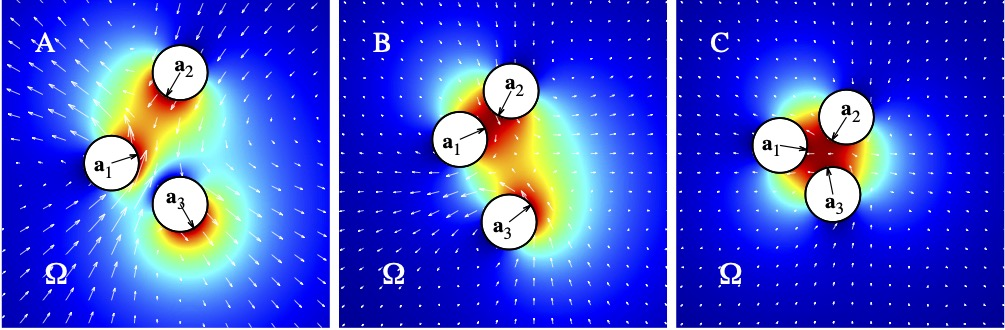
\includegraphics[width=0.55\textwidth]{figures/SpecificAim1/3Particles.jpg}
 \caption{\label{fig:3particles}
   \footnotesize
   Particles translate and rotate to lower the free energy $F[u]$
   subject to \eqref{eq:SL}, $f(u) = u^2$, and reach a minimal configuration in
   panel C. The colormap is blue for $u = 0$ and red for $u = 1$.
   The arrows are the velocity field $\mathbf{u}$.
 }
\end{wrapfigure}
The stress~\eqref{eq:stress} was first
introduced by~\cite{Fu2018_SIAM} and is the higher-dimensional
generalization of disjoining pressure \cite{MaRa76, ErLjCl89, KoNa15,
Nagle17, KUZMIN2005}. It is the mathematical ingredient responsible for
forming particle aggregates that sequester their hydrophobic surface
regions (Figure \ref{fig:3particles}).

%By solving the above system, we obtain translational and angular
%velocities of the many-body system. A second-order Adams-Bashforth
%scheme updates the particle positions and orientations.

The formulation presents a number of mathematical and numerical
challenges. For one, the domain is constantly changing so that a new
boundary value problem must be solved at each time step. The particle
boundaries are nearly touching and high-order numerical
schemes and adaptively chosen time-step sizes
are required to calculate trajectories accurately.
Furthermore, the domain is unbounded and care must be taken 
in capturing the far-field boundary conditions correctly. 
Finally, the numerical routine must handle large system sizes
efficiently.

%and
%\begin{equation}
%  \label{eq:force}
%  \int_{\Gamma_i} \ssigma \cdot \nnu \, \dif s = \FF_i,\quad 
%  \int_{\Gamma_i} (\xx - \aa_i)^{\perp} \cdot (\ssigma \cdot \nnu) \,
%  \dif s = T_i, \qquad i=1,\ldots,N_b,
%\end{equation}
%where
%$\ssigma = -p \mathbf{I} + \mu \left(\nabla \uu + \nabla \uu^T \right)$
%is the hydrodynamic stress tensor (pressure tensor) and $\nnu$ is the
%particle outward normal.

\subsection{Boundary Integral formulation}
\textbf{Take from prior years proposal}


\subsection{Outline of the proposal}
